\documentclass[11pt, letterpaper]{report}
\usepackage[T1]{fontenc}
\usepackage[pdftex]{graphicx}
\usepackage{amsmath}
\usepackage{algorithm}
\usepackage{algorithmic}
\usepackage{hyperref}
\usepackage[top=2.5cm,bottom=2.5cm,right=2.5cm,left=2.5cm]{geometry}
\usepackage{color}
\usepackage{listings}
\lstset{
	language=C++,
	keywordstyle=\bfseries\ttfamily\color[rgb]{0,0,1},
	identifierstyle=\ttfamily,
	commentstyle=\color[rgb]{0.133,0.545,0.133},
	stringstyle=\ttfamily\color[rgb]{0.627,0.126,0.941},
	showstringspaces=false,
	basicstyle=\small,
%	numberstyle=\footnotesize,
%	numbers=left,
%	stepnumber=1,
	numbersep=10pt,
	tabsize=2,
	breaklines=true,
	prebreak = \raisebox{0ex}[0ex][0ex]{\ensuremath{\hookleftarrow}},
	breakatwhitespace=false,
	aboveskip={1.5\baselineskip},
  columns=fixed,
  upquote=true,
  extendedchars=true,
% frame=single,
% backgroundcolor=\color{lbcolor},
}

\title{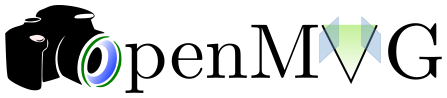
\includegraphics{../logo/openMVG_Logo.pdf}\newline
openMVG: Library reference
}
\author{Pierre MOULON}

\begin{document}
\maketitle
\newpage
\tableofcontents
\newpage

%%%%%%%%%%%%%%%%%%%%%%%
%%--
%%%%%%%%%%%%%%%%%%%%%%%
\chapter{Introduction}

\paragraph{}
OpenMVG (Multiple View Geometry) is a library for computer-vision scientists and especially targeted to the Multiple View Geometry community. It is designed to provide an easy access to the classical problem solvers in Multiple View Geometry and solve them accurately..

\subsection*{Why another library}
The openMVG credo is: "Keep it simple, keep it maintainable". OpenMVG targets readable code that is easy to use and modify by the community.\newline

All the features and modules are unit tested. This test driven development ensures that the code works as it should and enables more consistent repeatability. Furthermore, it makes it easier for the user to understand and learn the given features.

\subsection*{Acknowledgements}

openMVG authors would like to thank \href{http://code.google.com/p/libmv/}{libmv} authors for providing an inspiring base to design the openMVG library. Authors also would like to thank \href{http://www.mikrosimage.eu/}{Mikros Image} and \href{http://imagine.enpc.fr/}{LIGM-Imagine laboratory} for support and authorization to make this library as an open-source project.

\section*{License}

openMVG library is release under the \href{http://www.mozilla.org/MPL/2.0/}{MPL2} (Mozilla Public License 2.0). It integrates some sub-part under the MIT (Massachusetts Institute of Technology) and the BSD (Berkeley Software Distribution) license. Please refer to the license file contained in the source for complete license description.

\section*{Dependencies}

OpenMVG come as a standalone distribution, you don't need to install libraries to make it compiles and run. Exception for the Linux library is made for the png, zlib and jpeg library in order to use the one of the system.

%%%%%%%%%%%%%%%%%%%%%%%
%%--
%%%%%%%%%%%%%%%%%%%%%%%
\newpage
\chapter{The openMVG library}
\paragraph{}
The openMVG library is cut in various modules:
\begin{itemize}
\item image,
\item multiview,
\item robust\_estimation,
\item features,
\item matching,
\item numeric,
\item tracks.
\end{itemize}

The main contribution of the openMVG library is the multiview and robust\_estimation libraries that allow to handle easily Multiple View Geometry related task. The other libraries provide a common framework for all the samples that the user is free to use if desired.

%%%%%%%%%%%%%%%%%%%%%%%
%%--
%%%%%%%%%%%%%%%%%%%%%%%
\newpage
\chapter{Pinhole camera geometry}
\paragraph{}
A camera could be approximated by a projective model, often called pinhole projection. The simplest representation of a camera is a light sensible surface (sensor): an image plane, a lens (projective projection) and by a position in space.

\begin{center}
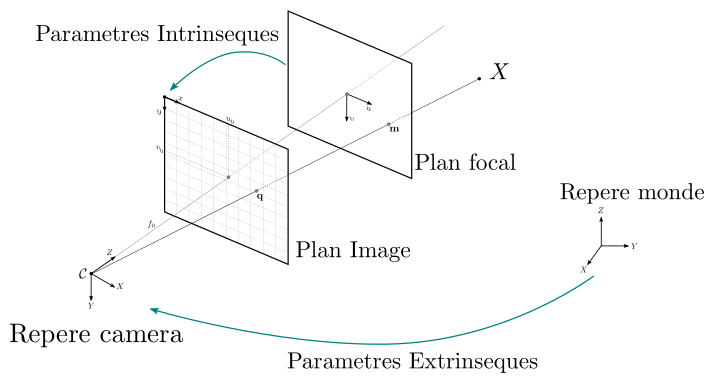
\includegraphics[scale=.6]{figures/pinhole_geometry}
\end{center}


The pinhole camera geometry models the projective camera with two sub-parametrizations, intrinsic and extrinsic parameters. Intrinsic parameters model the optic component (without distortion) and extrinsic model the camera position and orientation in space.

This projection of the camera is described as:
\begin{equation}
P_{3 \times 4} =
\begin{bmatrix}
f*k_u &  & c_u \\
 & f*k_v & c_v \\
 &  & 1
\end{bmatrix}
\begin{bmatrix}
 &  &  & t_x \\
 & R_{3 \times 3} &  & t_y \\
  &  &  & t_z \\
  0 & 0 & 0 & 1\\
\end{bmatrix}
\end{equation}

\begin{itemize}
\item Intrinsic parameters $[f, c_u, c_v]$:
\subitem $k_u$, $k_v$ : scale factor relating pixels to distance (often equal to $1$ or $height/width$  sensor ratio),
\subitem $f$ : the focal distance (distance between focal and image plane),
\subitem $c_u$, $c_v$ : the principal point, which would be ideally in the centre of the image.
\item Extrinsic parameters $[R|t] = [R|-R C]$:
\subitem $R$ : the rotation of the camera to the world frame,
\subitem $t$ : the translation of the camera. $t$ is not the position of the camera. It is the position of the origin of the world coordinate system expressed in coordinates of the camera-centred coordinate system. The position, $C$, of the camera expressed in world coordinates is~$C=-R^{-1} t = R^T t$~(since $R$ is a rotation matrix).
\end{itemize}

\paragraph*{}
A 3D point is projected in a image with the following formula (homogeneous coordinates):
\begin{center}
$ x_i = P X_i = K[R|t] X_i$
\end{center}

\begin{equation}
\begin{bmatrix}
u_i\\
v_i\\
w_i\\
\end{bmatrix} =
\begin{bmatrix}
f*k_u &  & c_u \\
 & f*k_v & c_v \\
 &  & 1\\
\end{bmatrix}
\begin{bmatrix}
 &  &  & t_x \\
 & R_{3 \times 3} &  & t_y \\
 &  &  & t_z \\
 0 & 0 & 0 & 1\\
\end{bmatrix}
\begin{bmatrix}
X_i\\
Y_i\\
Z_i\\
W_i\\
\end{bmatrix}
\end{equation}

%%%%%%%%%%%%%%%%%%%%%%%
%%--
%%%%%%%%%%%%%%%%%%%%%%%
\newpage
\chapter{openMVG multiview}
\paragraph{}
The multiview module consists of a collection of:
\begin{itemize}
\item solvers for 2 to n-view geometry constraints that arise in multiple view geometry,
\item a generic framework that can embed these solvers for robust estimation. It uses a concept called "kernel", explained later in this section.


\section{Two-view geometric estimation:}
openMVG provides solver for the following problems:
\begin{itemize}
\item affine,
\item homographic,
\item fundamental,
\subitem 7 to n pt,
\subitem 8 to n pt.
\item essential,
\subitem 8 to n pt,
\subitem 5pt + intrinsic.
\end{itemize}



\newpage
\subsection{Homography matrix:}

The homography matrix map the relation between two projection of a plane. It is a $(3\times3)$ matrix that links coordinates in left and right images with the following relation \ref{homography_eq}. Implementation follows the DLT (Direct Linear Transform) explain in~\cite{Hartley2004} book.

\begin{equation}
x_i^{\prime} = H x_i
\label{homography_eq}
\end{equation}

\begin{figure}[h!]
\begin{center}
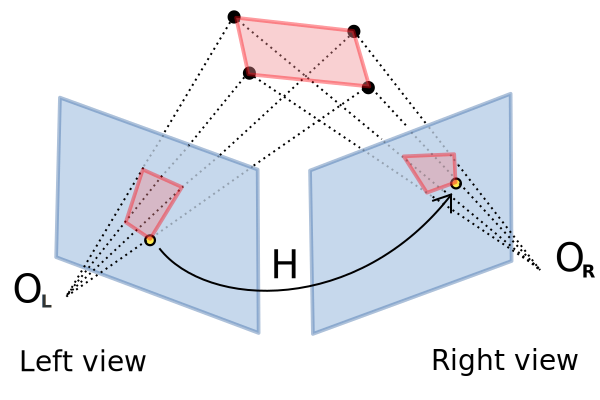
\includegraphics[scale=.5]{figures/Homography_geometry}
\caption{The homography matrix and the point to point constraint.}
\end{center}
\end{figure}

\newpage
\subsection{Fundamental matrix:}
The fundamental matrix is a relation between two image viewing the same scene where points projection are visible in the two images. Given a point correspondence between two view: $x_i=(u_i,v_i,1)^T$ and $x_i^\prime=(u_i^\prime,v_i^\prime,1)^T$, we obtain the following relation:
\begin{equation}
x_i^{\prime T}F x_i=0
\end{equation}

F is the $(3\times3)$ Fundamental matrix, it put in relation a point $x$ to a line where belong the projection of the 3D $X$ point. $l_i^\prime=Fx_i$ design the epipolar line on which the point $x_i'$ could be. The relation $x_i'^TFx_i=0$ exists for all corresponding point belonging to a stereo pair.

\begin{figure}[h!]
\begin{center}
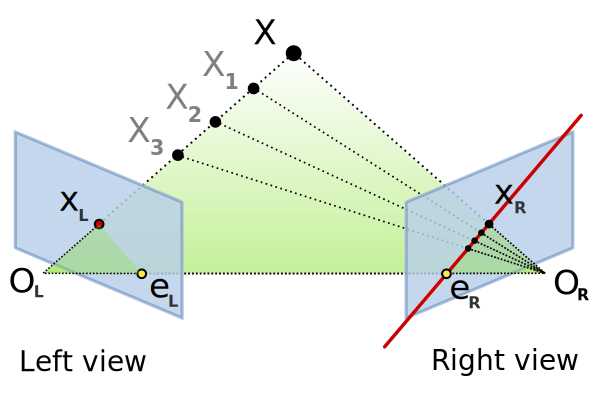
\includegraphics[scale=.5]{figures/Epipolar_geometry}
\caption{The fundamental matrix and the point to line constraint.}
\end{center}
\end{figure}

The fundamental matrix is sometime called bifocal-tensor, it is a \textbf{$3 \times 3$} matrix of rank $2$ with $7$ degree of freedom. $8$ ou $7$ correspondences are sufficient to computes the $F$ matrix. Implementation follows the DLT (Direct Linear Transform) explain in~\cite{Hartley2004} book.

\newpage
\subsection{Essential matrix}

Adding intrinsic parameter to the fundamental matrix gives a metric "object" that provide the following relation $E = K'^T F K$, this is the Essential relation explained by Longuet-Higgins in 1981~ \cite{LonguetHiggins81}. This essential matrix links the relative position of the camera to the fundamental matrix relation.

\begin{equation}
E = R [t]\times = K'^T F K
\end{equation}

\begin{figure}[h!]
\begin{center}
\includegraphics[scale=.6]{figures/essential_geometry}
\caption{Essential matrix.}
\end{center}
\end{figure}

\newpage
\subsection{Kernel concept}
A kernel is an association of data points, a model solver and an error estimator, i.e: \ref{kernel_concept_fig}.
\end{itemize}

\begin{figure}[h!]
\begin{center}
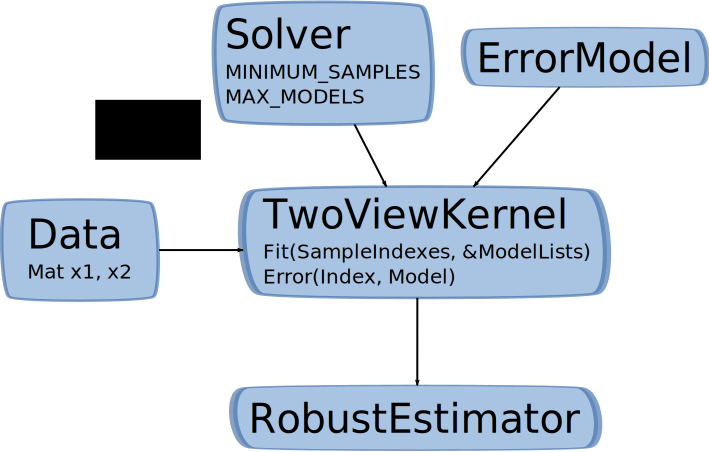
\includegraphics[scale=.5]{figures/kernel_concept}
\caption{The Kernel concept (the two view case).}
\label{kernel_concept_fig}
\end{center}
\end{figure}

\begin{description}
\item[Solver:]~\\
\subitem MINIMUM\_SAMPLES: The minimal number of point required for the model estimation,
\subitem MAX\_MODELS: The number of models that the minimal solver could return,
\subitem A Solve function that estimates a model from MINIMUM\_SAMPLES to $n$ vector data.
\item[ErrorModel:] An Error function that return the error of a sample data to the provided model.\\
\item[Kernel:] Embed data (putative), the model estimator and the error model.\\
\subitem This kernel is core brick used in the openMVG robust estimator framework.
\end{description}

%%%%%%%%%%%%%%%%%%%%%%%
%%--
%%%%%%%%%%%%%%%%%%%%%%%
\newpage
\chapter{3D-2D geometric constraint:}
\paragraph{}
openMVG provides solver for the following problems:
\begin{itemize}
\item pose estimation/ camera resection,
\subitem 6pt~\cite{Hartley2004},
\subitem 4pt with intrinsic EPnP~\cite{DBLP:journals/ijcv/LepetitMF09},
\subitem 3pt with intrinsic P3P~\cite{DBLP:conf/cvpr/KneipSS11}.
\end{itemize}

\newpage
\section{Camera resection/pose estimation:}
Given a serie of 3D-2D image plane correspondences it's possible to compute a camera pose estimation (i.e. Fig. \ref{resection_fig}). It consists in estimating the camera parameter of the right camera that minimize the residual error of the 3D points re-projections (see Fig.~\ref{residual_fig}), it's an optimization problem that trying to solve $P$ parameter in order to minimize $min \sum\limits_{i=1}^n x_i - P(X_i)$.

\begin{figure}[h!]
\begin{center}
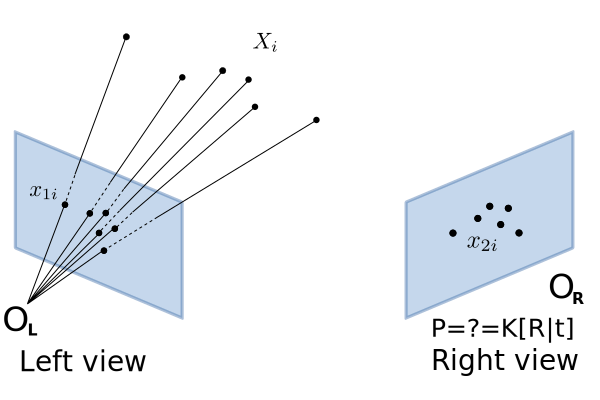
\includegraphics[scale=.6]{figures/resection_geometry}
\caption{Resection/Pose estimation from 3D-2D correspondences.}
\label{resection_fig}
\end{center}
\end{figure}

\begin{figure}[h!]
\begin{center}
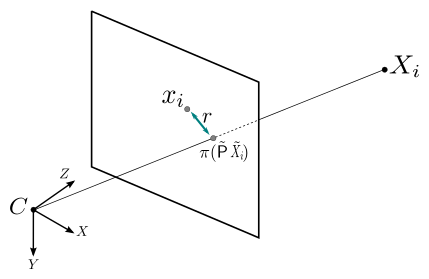
\includegraphics[scale=.4]{figures/residual_error}
\caption{Residual error.}
\label{residual_fig}
\end{center}
\end{figure}

%%%%%%%%%%%%%%%%%%%%%%%
%%--
%%%%%%%%%%%%%%%%%%%%%%%
\newpage
\chapter{Triangulation:}
\begin{itemize}
\item 2 views,
\newline
\begin{center}
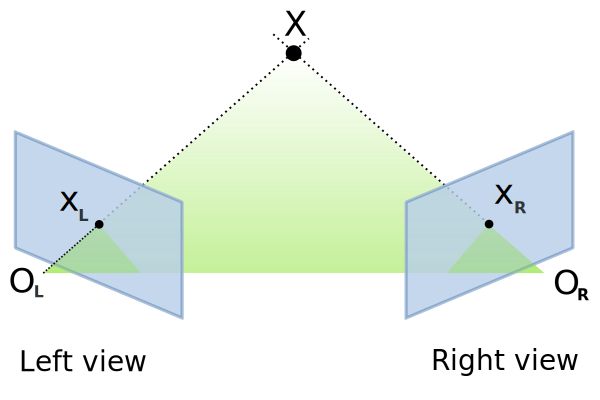
\includegraphics[scale=.5]{figures/triangulation_geometry}
\end{center}
\item N-views
\newline
\begin{center}
\includegraphics[scale=.6]{figures/triangulation_n_geometry}
\end{center}
% Nice illustration could be found here:
%http://archimede.bibl.ulaval.ca/archimede/fichiers/25229/ch06.html
\end{itemize}

%%%%%%%%%%%%%%%%%%%%%%%
%%--
%%%%%%%%%%%%%%%%%%%%%%%
\newpage
\chapter{openMVG robust estimation:}

\paragraph{}
Performing model estimation is not an easy task, data are always corrupted by noise and "false/outlier" data so robust estimation is required to find the "best" model along the possible ones.

\begin{figure}[h!]
\begin{center}
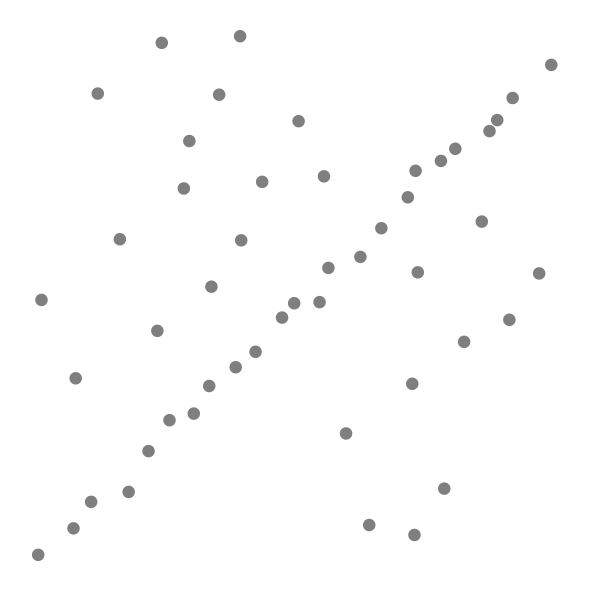
\includegraphics[scale=.3]{figures/robust_estimation_line}
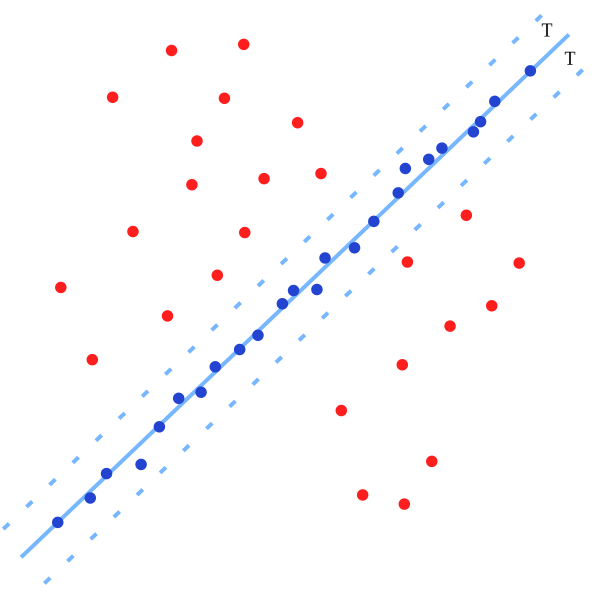
\includegraphics[scale=.3]{figures/robust_estimation_fitted_line}
\caption{Robust estimation: Looking for a line in corrupted data.}
\end{center}
\end{figure}


openMVG provides many methods to estimate one of the best possible model in corrupted data:
\begin{itemize}
\item Max-Consensus,
\item Ransac,
\item LMeds,
\item AC-Ransac (A Contrario Ransac)
\end{itemize}

\newpage
\section{Max-Consensus}
The idea of Max-Consensus is to use a random picked subset of data to find a model and test if this model is good or not the whole dataset. At the end you keep the model that best fit your cost function. Best fit defined as the number of data correspondences to the model under your specified threshold $T$.

\begin{algorithm}
\caption{~~Max-Consensus}
\begin{algorithmic}\label{algo:Max-Consensus}
\REQUIRE correspondences
\REQUIRE model solver, residual error computation
\REQUIRE $T$ threshold for inlier/outlier discrimination
\REQUIRE $maxIter$ the number of performed model estimation
\ENSURE inlier list
\ENSURE best estimated model $M_{best}$
\FOR{$i = 0 \to maxIter$}
\STATE Pick $N_{Sample}$ random samples
\STATE Evaluate the model $M_i$ for the random samples
\STATE Compute residuals for the estimated model
\IF {$Cardinal(residual<T) > previousInlierCount$}
\STATE $previousInlierCount = Cardinal(residual<T)$
\STATE $M_{best} = M_i$
\ENDIF
\ENDFOR
\end{algorithmic}
\end{algorithm}

Here an example of how find a best fit line:
\vspace{-.5cm}
\begin{lstlisting}
Mat2X xy(2, 5);
// Defines some data points
xy << 1, 2, 3, 4,  5, // x 
      3, 5, 7, 9, 11; // y

// The base model estimator and associated error metric
LineKernel kernel(xy);

// Call the Max-Consensus routine
std::vector<size_t> vec_inliers;
Vec2 model = MaxConsensus(kernel, ScorerEvaluator<LineKernel>(0.3), &vec_inliers);
\end{lstlisting}

\newpage
\section{Ransac}
Ransac~\cite{DBLP:journals/cacm/FischlerB81} is an evolution of Max-Consensus with a-priori information about the noise and corrupted data amount of the data. Those informations allow to reduce the number of iteration in order to be sure to have made sufficient random sampling steps in order to find the model for the given data confidence. The number of remaining steps is so iteratively updated given the inlier/outlier ratio of the current found model.

~\newline
Here an example of how find a best fit line:
\vspace{-.5cm}
\begin{lstlisting}
Mat2X xy(2, 5);
// Defines some data points
xy << 1, 2, 3, 4,  5, // x 
      3, 5, 7, 9, 11; // y

// The base model estimator and associated error metric
LineKernel kernel(xy);

// Call the Ransac routine
std::vector<size_t> vec_inliers;
Vec2 model = Ransac(kernel, ScorerEvaluator<LineKernel>(0.3), &vec_inliers);
\end{lstlisting}

\newpage
\section{AC-Ransac A Contrario Ransac}

RANSAC requires the choice of a threshold $T$, which must be balanced:
\begin{itemize}
\item Too small: Too few inliers, leading to model imprecision,
\item Too large: Models are contaminated by outliers (false data).
\end{itemize}

AC-Ransac~\cite{MOULON/ACCV12} uses the \emph{a~contrario} methodology in order to find a model that best fits the data with a confidence threshold $T$ that adapts automatically to noise. It so find a model and it's associated noise. If there is too much noise, the \emph{a~contrario} methods return that no model was found.

\begin{figure}[h!]
\begin{center}
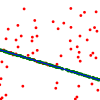
\includegraphics[width=.2\linewidth]{figures/ac_ransac/0_3_line_robust}\hspace{1em}
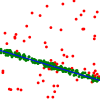
\includegraphics[width=.2\linewidth]{figures/ac_ransac/1_8_line_robust}\hspace{1em}
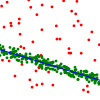
\includegraphics[width=.2\linewidth]{figures/ac_ransac/2_7_line_robust}\hspace{1em}
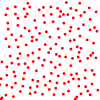
\includegraphics[width=.2\linewidth]{figures/ac_ransac/tooNoisy_line_robust}\hfill
\caption{\emph{a~contrario} robust estimation, noise adaptivity.}
\end{center}
\end{figure}

~\newline
Here an example of how find a best fit line, by using the {\em a contrario} robust estimation framework:
It's a bit more complex, we use a class in order to perform the {\em a contrario} required task.

\vspace{-.5cm}
\begin{lstlisting}
Mat2X xy(2, 5);
// Defines some data points
xy << 1, 2, 3, 4,  5, // x 
      3, 5, 7, 9, 11; // y

// The a contrario adapted base model estimator and associated error metric
const size_t image_width = 12;
ACRANSACOneViewKernel<LineSolver, pointToLineError, Vec2> lineKernel(xy, image_width, image_width);

// Call the AC-Ransac routine
std::vector<size_t> vec_inliers;
Vec2 line;
std::pair<double,double> res= ACRANSAC(lineKernel, vec_inliers, 300, &line);
double dPrecision = res.first;
double dNfa = res.second;
\end{lstlisting}

%%%%%%%%%%%%%%%%%%%%%%%
%%--
%%%%%%%%%%%%%%%%%%%%%%%
\newpage
\chapter{openMVG image:}
\paragraph{}
This module provides generic algorithms for image related tasks:
\begin{description}
\item[Container] A generic image container:
\subitem Template pixel type: gray, RGB, RGBA,
\subitem User specified bit depth, uchar, float, double.
\item[Image I/O] Loading, writing:
\subitem ppm/pgm, jpeg, png
\item[Drawing operations] ~
\subitem lines,
\subitem circles,
\subitem ellipses.
\end{description}

%%%%%%%%%%%%%%%%%%%%%%%
%%--
%%%%%%%%%%%%%%%%%%%%%%%
\newpage
\chapter{openMVG matching:}
\paragraph{}
A generic interface to perform K-Nearest Neighbor search:
\begin{itemize}
\item Brute force,
\item Approximate Nearest Neighbor (FLANN~\cite{muja_flann_2009}).
\end{itemize}

This module works for any size of data, it could be use to match 128, 64, vector long descriptors or to find closest 3D points. The used metric is customizable and enable matching under L2 or a user customized distance (L1, ...). The Nearest Neighbor retrieval allows to retrieve the N nearest points and so to perform easily the "Nearest Neighbor Distance Ratio" distance check to remove repetitive elements.

%%%%%%%%%%%%%%%%%%%%%%%
%%--
%%%%%%%%%%%%%%%%%%%%%%%
\newpage
\chapter{openMVG tracks:}
\paragraph{}
The problem of feature points tracking is to follow the position of a characteristic point in a set of images. These multi-view correspondences are called \emph{tracks}. Track identification in a set of images (ordered, or not) is an important task in computer vision. It allows solving geometry-related problems like video stabilization, tracking, match-moving, image-stitching, structure from motion and odometry.

\subparagraph{The "track" computation problem.}
Considering $n$ pairwise feature correspondences as input we want sets of corresponding matching features across multiple images, as illustrated in Figures~\ref{fig:tracks_intro},~\ref{fig:tracks} with video frames.

\noindent
\begin{figure}[h!]
\begin{center}
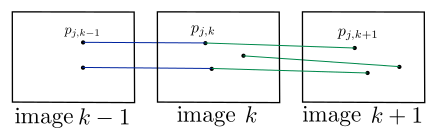
\includegraphics[scale=.6]{figures/feat_tracking/Tracks}
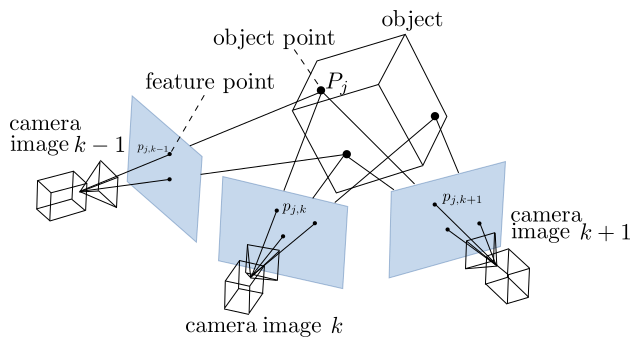
\includegraphics[scale=.4]{figures/SfM_geometry.pdf}
\includegraphics[scale=.22]{figures/feat_tracking/feat_Tracking}
\caption{From features to tracks}
\label{fig:tracks_intro}
\end{center}
\end{figure}

\newpage
The openMVG library provides an efficient solution to solve the union of all the pairwise correspondences. It is the implementation of the CVMP12 paper "Unordered feature tracking made fast and easy"~\cite{MOULON/CVMP12}.

\begin{figure} [h!]
\begin{center}
\includegraphics[scale=.38]{figures/feat_tracking/feat_Tracking_illus.jpeg}
\caption{Feature based tracking.}
\label{fig:tracks}
\end{center}
\end{figure}

Some comments about the data structure:
\vspace{-.5cm}
\begin{lstlisting}
// Data structure to store a track: collection of {ImageId,FeatureId}
//   The corresponding image points with their imageId and FeatureId.
typedef std::map<size_t,size_t> submapTrack;
// A track is a collection of {trackId, submapTrack}
typedef std::map< size_t, submapTrack > STLMAPTracks;

STLMAPTracks map_tracks;

// In order to visit all the tracks, follow this code:
for (tracks::STLMAPTracks::const_iterator iterT = map_tracks.begin();
  iterT != map_tracks.end(); ++ iterT)
{
 const size_t trackId = iterT->first;
 const tracks::submapTrack & track = iterT->second;
 for( tracks::submapTrack::const_iterator iterTrack = track.begin();
   iterTrack != track.end(); ++iterTrack)
 {
   size_t imageId = iterTrack->first;
   size_t featId = iterTrack->second;
   
   // Get the feature point
 }
}
\end{lstlisting}

%%%%%%%%%%%%%%%%%%%%%%%
%%--
%%%%%%%%%%%%%%%%%%%%%%%
\newpage
\chapter{Vector drawing:}
\paragraph{}
openMVG considers that visualizing data is important. OpenMVG provides a class that help to perform vector graphics (SVG) drawing in order to have the best possible visualization of his algorithm output. Vector graphics allows keeping details when you zoom what is not done when you use raster graphics. (SVG files are supported by web navigator and the Inkscape software).

\vspace{-.5cm}
\begin{lstlisting}
// Draw a cardiod curve with the svg polyline
// http://en.wikipedia.org/wiki/Cardioid
  { // Pre-compute (x,y) curve points
    size_t nbPoints = 120;
    std::vector<float> vec_x(nbPoints, 0.f), vec_y(nbPoints, 0.f);
    double S = 20.;
    for (size_t i = 0; i < nbPoints; ++i) {
      const double theta = i * 2 * M_PI / nbPoints;
      //-- Cardioid equation
      vec_x[i] = (3*S + S*(2.*sin(theta)-(sin(2.*theta))));
      vec_y[i] = (2*S - S*(2.*cos(theta)-(cos(2.*theta))));
    }
    // Create a svg surface and add the cardiod polyline
    svgDrawer svgSurface(6*S, 6*S); //Create a svg object
    svgSurface.drawPolyline(
      vec_x.begin(), vec_x.end(),
      vec_y.begin(), vec_y.end(),
      svgStyle().stroke("blue", 2));

    //Export the SVG stream to a file
    std::string sFileName = "ThirdExample.svg";
    std::ofstream svgFile(sFileName.c_str());
    svgFile << svgSurface.closeSvgFile().str();
    svgFile.close();
  }
\end{lstlisting}
Here the result exported vector graphic:
\includegraphics[scale=1]{figures/vectorGraphics/ThirdExample}
  
%%%%%%%%%%%%%%%%%%%%%%%
%%--
%%%%%%%%%%%%%%%%%%%%%%%
\newpage
\chapter{3D point cloud handler:}
- PLY point cloud export (PLY is known as the Polygon File Format or the Stanford Triangle Format).\newline

Different interfaces have been written in order to export:
\begin{itemize}
\item Point cloud,
\item Coloured point cloud,
\item Camera location.
\end{itemize}

%%%%%%%%%%%%%%%%%%%%%%%
%%--
%%%%%%%%%%%%%%%%%%%%%%%
\newpage
\chapter{Structure from Motion:}

\paragraph{}
Structure from Motion (Fig.~\ref{fig:SfM}) computes an external camera pose per image (the motion) and a 3D point cloud (the structure) representing the pictured scene~(Fig.~\ref{fig:SfM_2}). Inputs are images and internal camera calibration information (intrinsic parameters). Feature points are detected in each image (e.g., SIFT) and matched between image pairs. There are two main approaches to correlate detected features and solve the SfM problem: the \textit{incremental} pipeline and the \textit{global} method.

\noindent
\begin{figure}[h!]
\begin{center}
\includegraphics[scale=.4]{figures/sfm/input_images.jpg}
\newline
\hfill
\includegraphics[scale=.46]{figures/sfm/sceaux_camLocation.jpg}
\hspace{1cm}
\includegraphics[scale=.21]{figures/sfm/sparse_Front.jpg}
\hfill
\end{center}
\caption{Input images, estimated camera location and structure.}
\label{fig:SfM_2}
\end{figure}

\newpage
openMVG proposes a customizable implementation of an Incremental Structure from Motion chain, it is the implementation use for the paper "Adaptive Structure from Motion with {\em a~contrario} model estimation"~\cite{MOULON/ACCV12} published at ACCV 2012.

\begin{figure}[h!]
\begin{center}
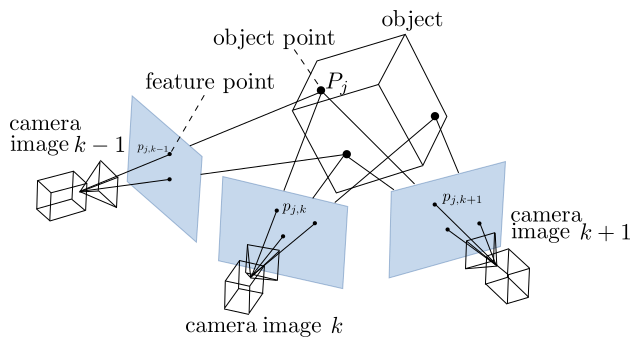
\includegraphics[scale=.6]{figures/SfM_geometry.pdf}
\caption{Structure from Motion.}
\label{fig:SfM}
\end{center}
\end{figure}

The incremental pipeline is a growing reconstruction process (i.e algorithm~\ref{algo:incremsfm}). It starts from an initial two-view reconstruction (the seed) that is iteratively extended by adding new views and 3D points, using pose estimation and triangulation. Due to the incremental nature of the process, successive steps of non-linear refinement, like Bundle Adjustment (BA) and Levenberg-Marquardt steps, are performed to minimize the accumulated error (drift). In this implementation we use the ceres-solver, a generic non-linear least squares problems solver~\cite{ceres-manual}, in order to perform Bundle Adjustment steps.\newline

\newpage
The general feature correspondence and SfM processes are described in algorithms \ref{algo:corresp} and~\ref{algo:incremsfm}. The first algorithm outputs pairwise correspondences that are consistent with the estimated fundamental matrix. The initial pair must be chosen with numerous correspondences while keeping a wide enough baseline. The second algorithm takes these correspondences as input and yields a 3D point cloud as well as the camera poses. Steps marked with a star~($*$) are estimated within the {\em a~contrario} framework. This allows critical thresholds to be automatically adapted to the input images (and remove the choice of an empiric $T$ threshold value).

\begin{algorithm}
\caption{~~Computation of geometry-consistent pairwise correspondences}
\begin{algorithmic}\label{algo:corresp} 
\REQUIRE image set
\ENSURE  pairwise point correspondences that are geometrically consistent
\STATE Compute putative matches:
\STATE \quad detect features in each image and build their descriptor
\STATE \quad match descriptors (brute force or approximate nearest neighbor)
\STATE Filter geometric-consistent matches:
\STATE \quad \mbox{}\llap{$*$~~\quad}estimate fundamental matrix $F$
\end{algorithmic}
\end{algorithm}

\begin{algorithm}
\caption{~~Incremental Structure from Motion}
\begin{algorithmic}\label{algo:incremsfm}
\REQUIRE internal camera calibration (matrix $K$, possibly from EXIF data)
\REQUIRE pairwise geometry consistent point correspondences
\ENSURE 3D point cloud
\ENSURE camera poses
\STATE compute correspondence tracks $t$
\STATE compute connectivity graph $G$ (1 node per view, 1 edge when enough matches)
\STATE pick an edge $e$ in $G$ with sufficient baseline
\STATE \mbox{}\llap{$*$~~}robustly estimate essential matrix from images of $e$
\STATE triangulate $t \cap e$, which provides an initial reconstruction
\STATE contract edge $e$
\WHILE{$G$ contains an edge}
\STATE pick edge $e$ in $G$ that maximizes track($e$) \(\cap\) $\{$3D points$\}$
\STATE \mbox{}\llap{$*$~~$\quad$}robustly estimate pose (external orientation/resection)
\STATE triangulate new tracks
\STATE contract edge $e$
\STATE perform bundle adjustment
\ENDWHILE
\end{algorithmic}
\end{algorithm}

\newpage
\paragraph{}
Once camera position and orientation have been computed, Multiple View Stereo-vision algorithms to compute a dense scene representation could be used. OpenMVG exports a PMVS~\cite{Furu:2010,Furu:2010:PMVS} ready to use data. Figure~\ref{fig:SfM_PMVS} shows an example on the scene of the figure~\ref{fig:SfM_2}.
\noindent
\begin{figure}[h!]
\begin{center}
\includegraphics[scale=.2]{figures/sfm/dense_Side.jpg}
\includegraphics[scale=.2]{figures/sfm/dense_Front.jpg}
\caption{Multiple View Stereo-vision densification on the estimated scene using PMVS \cite{Furu:2010,Furu:2010:PMVS}.}
\label{fig:SfM_PMVS}
\end{center}
\end{figure}

Tools to draw detected Keypoints, putative matches, geometric matches and tracks are provided along the SfM binary directory.

\newpage
\section{Structure from Motion chain usage}

The {\em a contrario} Structure from Motion chain take as input a sequence of \textbf{distortion corrected images} and the intrinsic associated calibration matrix $K$. This calibration matrix is stored as a "K.txt" file as a raw ascii $3\times3$ matrix in the same directory as the pictures.\\
Using a 3 directories based data organisation structure is suggested:
\begin{description}
\item[images] ~
\begin{itemize}
\item your image sequence,
\item K.txt
\end{itemize}
\item[matches] (the points and matches information will be saved here)
\item[outReconstruction] (directory where result and log of the 3D reconstruction will be exported)
\end{description}

\subsection*{Point matching:}
The first step consists in computing relative image matches~(i.e algorithm~\ref{algo:corresp}):
You have to use the \textit{openMVG\_main\_computeMatches} software in the software/SfM openMVG module.
\vspace{-.5cm}
\begin{lstlisting}
$ openMVG_main_computeMatches -i /home/pierre/Pictures/Dataset/images -e *.JPG -o /home/pierre/Pictures/Dataset/matches
\end{lstlisting}
Arguments are the following:
\begin{description}
\item[-i|--imadir] the path where image are stored.
\item[-e|--ext] image extension i.e "*.jpg" or "*.png". Case sensitive.
\item[-o|--outdir] path where features, descriptors, putative and geometric matches will be exported.
\item[-r|--distratio] optional argument (Nearest Neighbor distance ratio, default value is set to 0.6).
\item[-s|--octminus1] optional argument (Use the octave -1 option of SIFT or not, default value is set to false: 0).
\end{description}

Once matches have been computed you can, at your choice, display detected points, matches or start the 3D reconstruction.

\subsection*{Point, matching visualization:}

Three softwares are available to display:
\begin{description}
\item[Detected keypoints] \textit{openMVG\_main\_exportKeypoints}
\item[Putative, Geometric matches] \textit{openMVG\_main\_exportMatches}
\item[Tracks] \textit{openMVG\_main\_exportTracks}
\end{description}

\subsection*{SfM, 3D structure and camera calibration:}

The main binary in order to run the SfM process is \textit{openMVG\_main\_IncrementalSfM}, it use previous computed data and is implemented as explained in algorithm~\ref{algo:incremsfm}.
\vspace{-.5cm}
\begin{lstlisting}
$ openMVG_main_IncrementalSfM -i /home/pierre/Pictures/Dataset/images/ -m /home/pierre/Pictures/Dataset/matches/ -o /home/pierre/Pictures/Dataset/outReconstruction/
\end{lstlisting}

\textit{openMVG\_main\_IncrementalSfM} displays to you some initial pairs that share an important number of common point. Please select two image index and the 3D reconstruction will start.

\bibliographystyle{plain}
\bibliography{biblio}

\end{document}
